\subsection{Titulación}

  \paragraph{}Se procede a crear la titulación a la que pertenece el alumno,en
  este caso \textit{Grado de Bioquímica}, cuyo plan de estudios es del año 2000.
  Para ello, se realizará la creación de una nueva titulación, tal y como se
  describió en el capítulo \ref{addTitulacion}, \textit{Añadir titulación}.

  \paragraph{}Una vez que aparezca el formulario de creación, se debe introducir
  el nombre de la titulación, con lo que la pantalla quedaría tal y como refleja
  la figura \ref{ejemploAddTitulacion}.

  \begin{figure}[!ht]
    \begin{center}
      \fbox{
      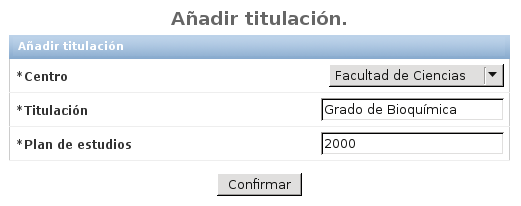
\includegraphics[scale=0.55]{5.Ejemplos_Practicos/5.3.IntroduccionDatos/5.3.2.Titulacion/add_titulacion.png}
      }
      \caption{Creación de \textit{Centro} de ejemplo.}
      \label{ejemploAddTitulacion}
    \end{center}
  \end{figure}

  \paragraph{}Una vez rellenado el formulario, se pulsará el botón
  \textit{Confirmar}, el cual se puede ver en la figura
  \ref{capturaBotonConfirmar}. Si el formulario rellenado es válido, y no tiene
  errores, se creará el nuevo elemento en el sistema. En caso de contener
  información no válida, un mensaje de error aparecerá indicando los campos
  del formulario que no han pasado la validación, los cuales habrá que modificar
  para introducir correctamente el elemento en el sistema.
